\renewcommand{\chaptername}{\scshape Partie}
\chapter{\normalfont \scshape Effet Schlieren}
\section{Principe du dispositif}
L'air est un fluide transparent, il possède un indice de réfraction qui suit une évolution linéaire par rapport à la masse volumique :
\begin{align}
	n = 1\,+\,k\,\rho
\end{align}
où $\mathnormal{n}$ est l'indice de réfraction du fluide, $\mathnormal{\rho}$ sa masse volumique et $\mathnormal{k}$ une constante appelée constante de Gladstone-Dale~\ref{ref:harvardedu}. Si $\mathnormal{n_i}$ et $\mathnormal{n_r}$ sont respectivement les indices de réfraction des rayons incident et réfléchi, $\mathnormal{\theta_i}$ l'angle d'incidence et $\mathnormal{\theta_r}$ l'angle de réfraction, on peut écrire la loi de \textsc{Snell-Descartes} :
\begin{align}
	n_i\times\,sin(\theta_i) = n_r\times\,sin(\theta_r) 
\end{align}
En faisant varier de manière non uniforme la température ou la pression de l'air, on fait apparaître des gradients de densité, ce qui fait que l'indice de réfraction ne varie pas de la même façon partout dans le fluide. Par conséquent, les rayons lumineux sont déviés, ce qui permet d'observer l'effet Schlieren. Le montage optique peut être réalisé avec un miroir sphérique ou avec deux lentilles convergentes.
\subsection{Dispositif avec miroir sphérique}
\begin{figure}[H]
	\centering
	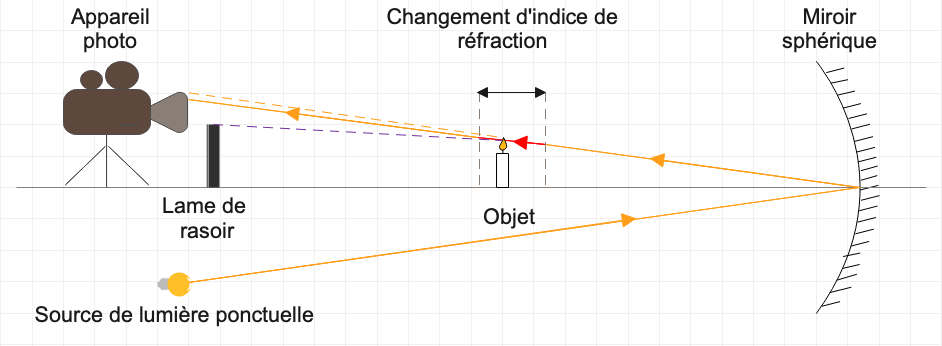
\includegraphics[scale = 0.4]{figures/schlieren_miroir.png}
	\caption{\small{\textit{Schéma du dispositif de Schlieren avec miroir sphérique}}}
	\label{fig:schlieren_miroir}
\end{figure}
Ce dispositif consiste en un miroir sphérique éclairé par une source ponctuelle ; un écran ou une caméra est placé à côté de cette dernière, toujours à une distance égale à deux fois la distance focale du miroir, pour capturer les rayons lumineux réfléchis. Or l’objet à observer est placé en face du miroir, créant une perturbation dans l’air. Certains rayons sont alors déviés, puis coupés par une lame de rasoir qui agit en tant que filtre. On observe ainsi des tâches plus ou moins sombres correspondant à la forme de la perturbation~\ref{ref:harvardedu}.
\subsection{Dispositif avec lentilles convergentes}
\begin{figure}[H]
	\centering
	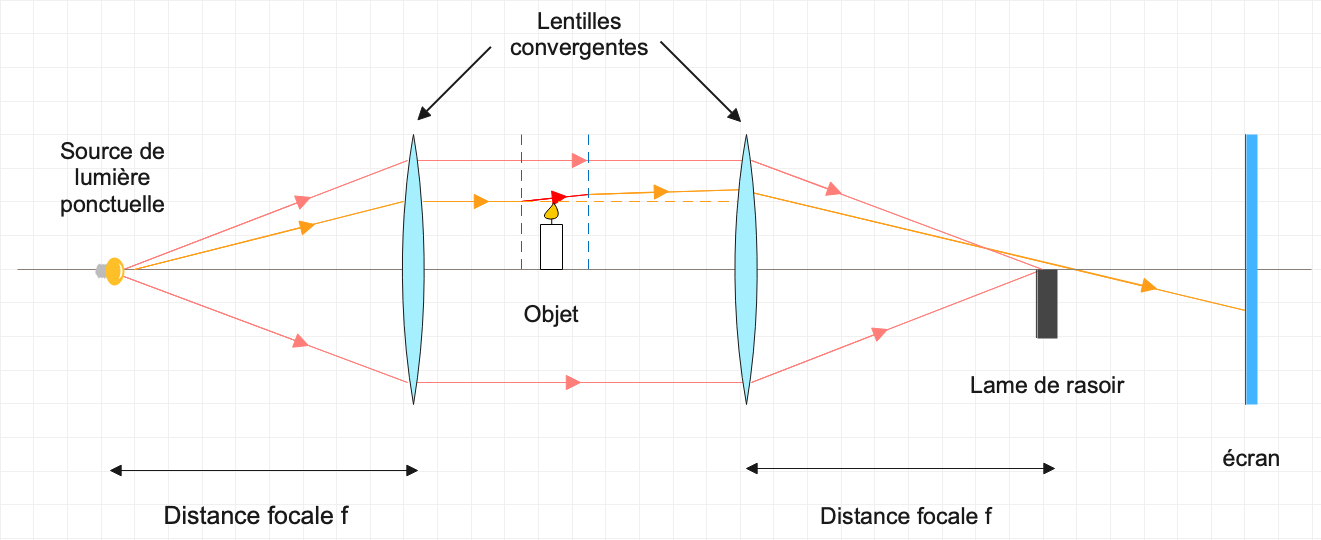
\includegraphics[scale = 0.3]{figures/schlieren_lentilles.png}
	\caption{\small{\textit{Schéma du dispositif de Schlieren avec lentilles convergentes}}}
	\label{fig:schlieren_lentilles}
\end{figure}
Ce système est constitué d'une source de lumière ponctuelle, d'une lame de rasoir, d'un écran et de deux lentilles convergentes faisant office de lentille de Fresnel. On positionne la source ponctuelle au point focal objet de l'une des lentilles afin d'obtenir un faisceau de rayons parallèles, et on se sert de l'autre lentille pour faire converger le faisceau, créant ainsi un système afocal. En plaçant la lame de rasoir au point focal image de la deuxième lentille, on élimine les rayons parallèles au faisceau, ce qui permet d'observer les rayons déviés par effet Schlieren sur l'écran.
\\
\\
Le but de cette première partie est donc de réussir à observer l'influence des gradients de densité sur l'air grâce à l'un des dispositifs énoncés précédemment.
\section{Protocole et organisation}
\subsection{Cahier des charges}
Une fois l'objectif défini, la mise en place d'un plan d'organisation s'est avérée judicieuse pour avancer dans le projet. Pour ce faire, le diagramme de GANTT de la figure~\ref{fig:gantt_schlieren} a été établi :
\begin{figure}[H]
	\centering
	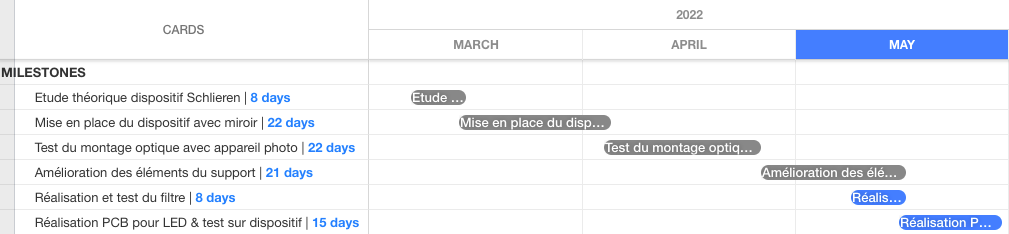
\includegraphics[scale = 0.43]{figures/gantt_schlieren.png}
	\caption{\small{\textit{Diagramme de GANTT prévu pour le montage optique}}}
	\label{fig:gantt_schlieren}
\end{figure}
Par ailleurs, parmi les sept membres du groupe, quatre ont été chargés de mettre en place le système optique, un rôle a été attribué à chacun des membres :
\begin{table}[H]
	\centering
	\setlength{\tabcolsep}{15pt}
	\begin{tabular}{|l l l l|}
		\hline
		\vtop{\hbox{\strut \small\textbf{Responsable}}\hbox{\strut \small\textbf{effet Schlieren}}}&\vtop{\hbox{\strut \small\textbf{Responsable}}\hbox{\strut \small\textbf{communication}}}&\vtop{\hbox{\strut \small\textbf{Responsable}}\hbox{\strut \small\textbf{technique}}}&\vtop{\hbox{\strut \small\textbf{Responsable}}\hbox{\strut \small\textbf{planning}}}\\
		\hline
		\vtop{\hbox{\strut \small{Yvonne}}\hbox{\strut \small{SAUTRIOT}}}&\vtop{\hbox{\strut \small{Léo}}\hbox{\strut \small{LAFFAY}}}&\vtop{\hbox{\strut \small{Alexandre}}\hbox{\strut \small{OCKIER}}}&\vtop{\hbox{\strut \small{Nada}}\hbox{\strut \small{KOUDDANE}}}\\
		\hline
	\end{tabular}
	\caption{\small\textit{Membres et tâches attribuées (dispositif à imagerie Schlieren)}}
	\label{fig:gestion_schlieren}
\end{table}
\subsection{Mise en place des montages optiques}
\subsubsection{\large\normalfont{\textsc{Montage avec lentilles convergentes}}}
Le système optique avec lentilles convergentes a été constitué à partir des éléments suivants :
\begin{itemize}
	\item Deux lentilles convergentes de distance focale \textbf{50 mm};
	\item Une lame de rasoir;
	\item Une source lumineuse : le flash d'un téléphone portable recouverte de papier aluminium;
	\item Un écran.
\end{itemize}
\subsubsection{\large\normalfont{\textsc{Montage avec miroir sphérique}}}
Pour ce montage, le matériel suivant a été utilisé :
\begin{itemize}
	\item Un miroir sphérique : \textbf{ø 86 mm}, distance focale : \textbf{260 mm};
	\item Une lame de rasoir;
	\item Une source lumineuse : lampe disponible en salle de TP ou flash de téléphone portable;
	\item Un appareil photo.
\end{itemize}
\begin{figure}[H]
	\centering
	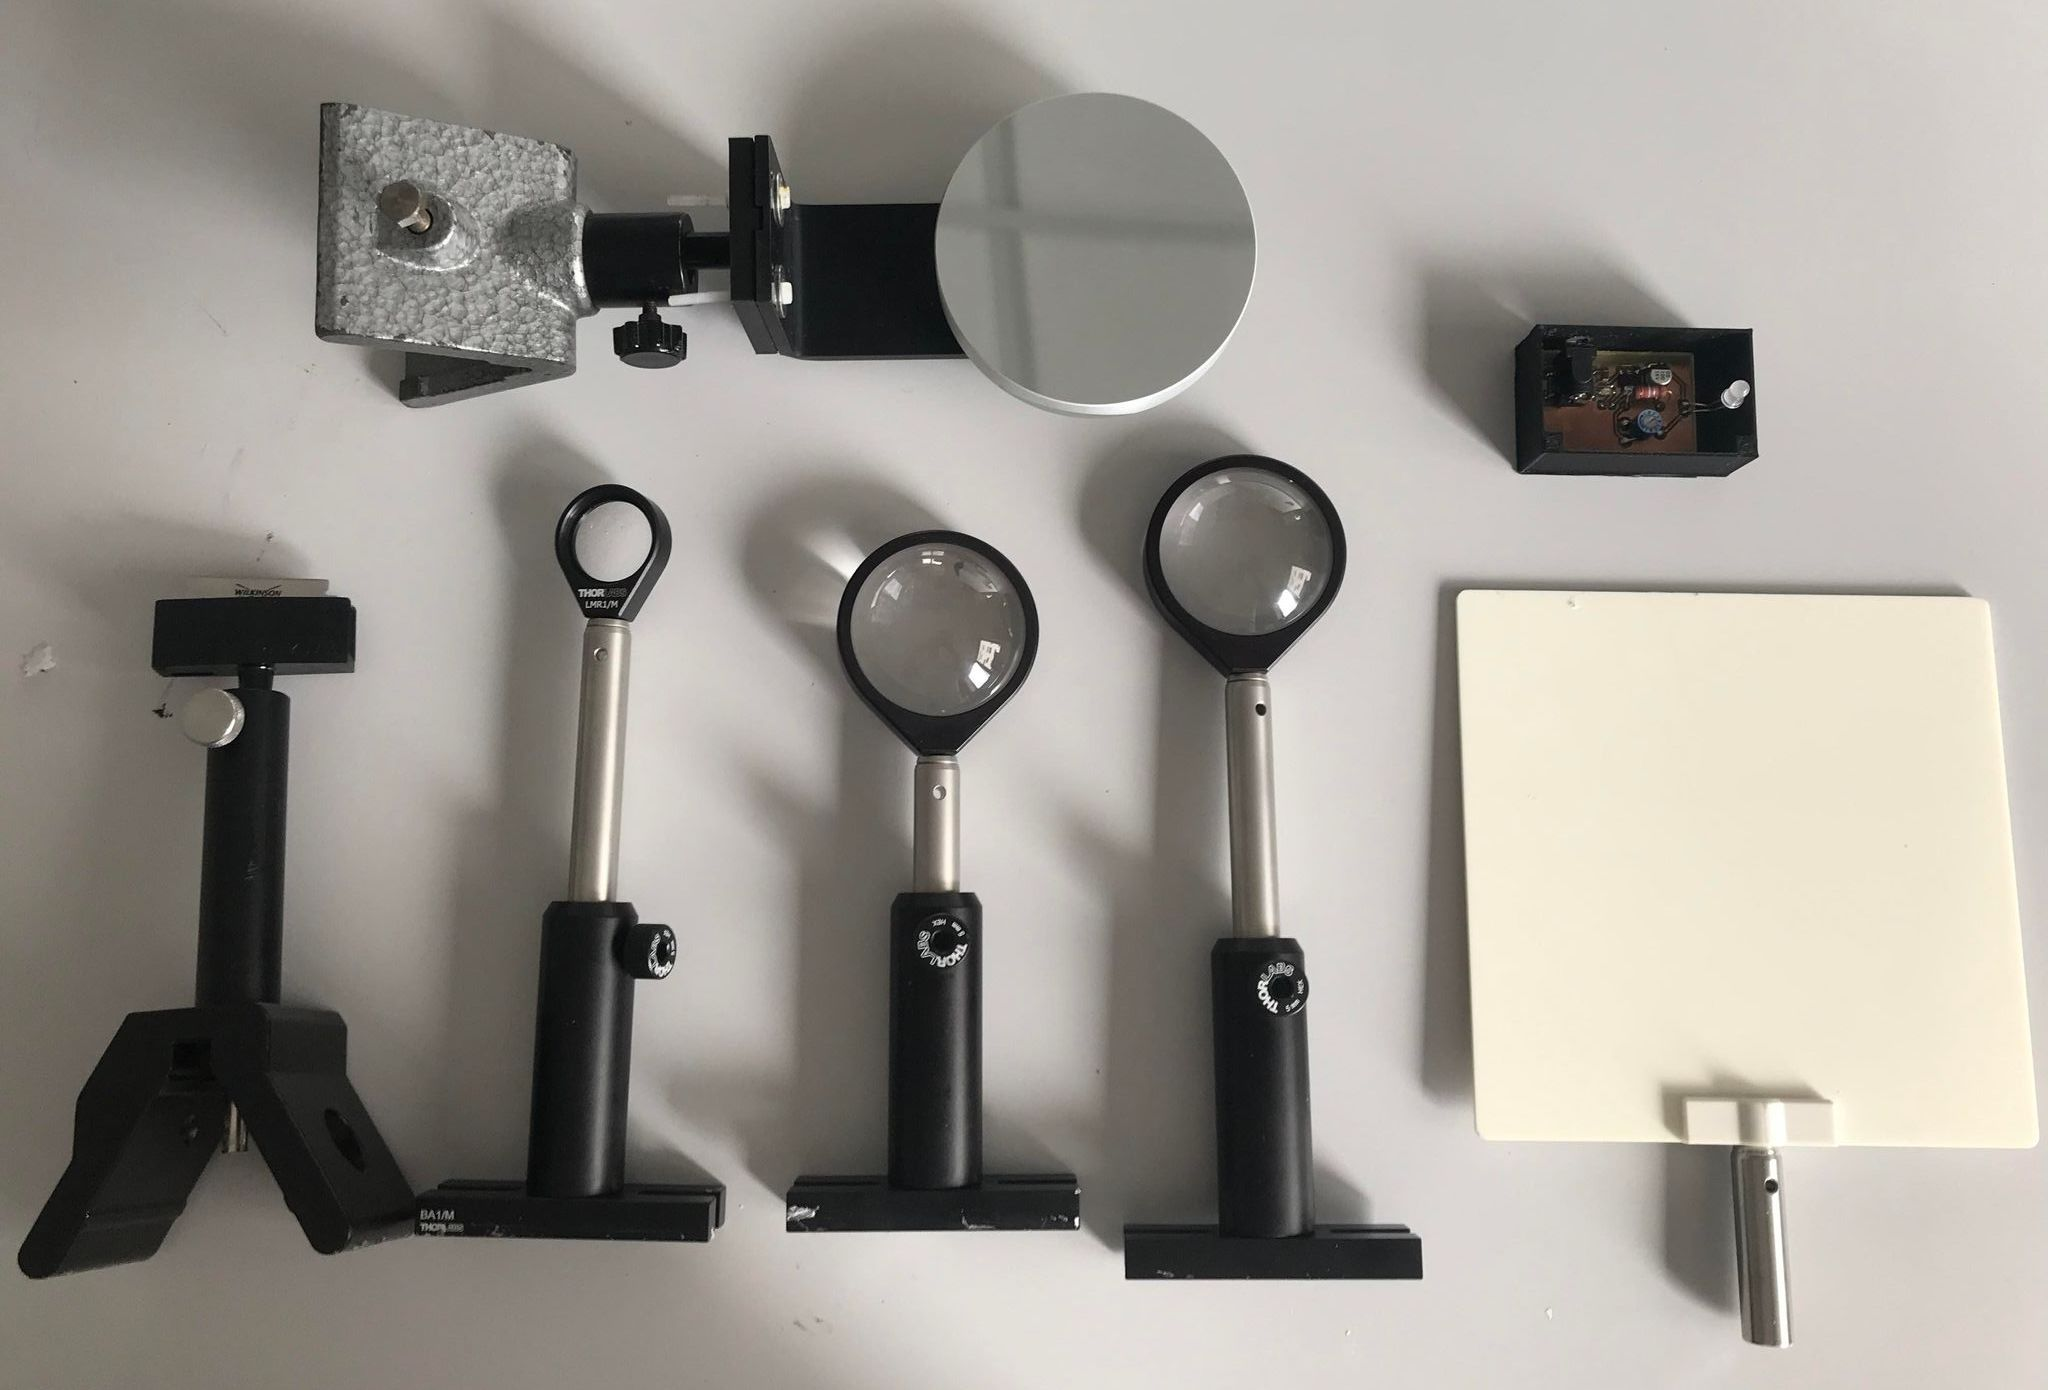
\includegraphics[scale = 0.12]{figures/materiel.jpg}
	\caption{\small{\textit{Matériel utilisé pour l'effet Schlieren}}}
	\label{fig:materiel}
\end{figure}
\subsection{Améliorations des montages}
\begin{figure}[H]
	\centering
	\begin{subfigure}[t]{0.49\textwidth}
		\centering
		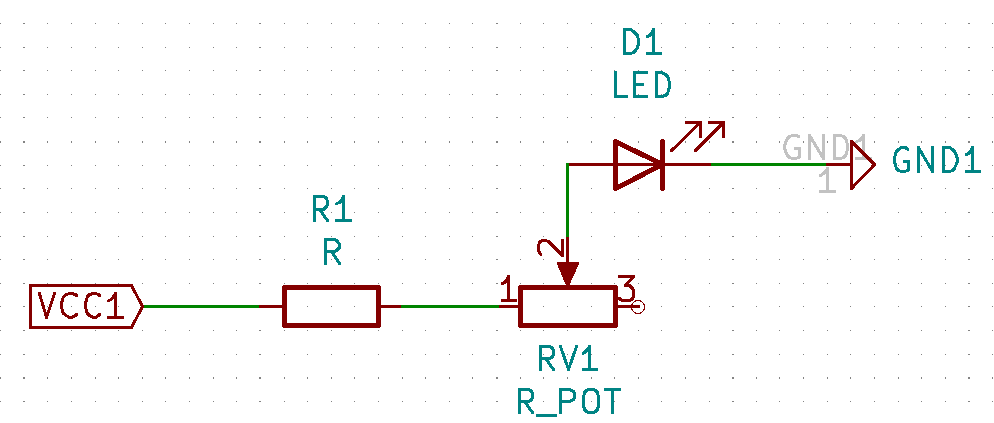
\includegraphics[scale=0.2]{figures/schema_kicad.png}
		\caption{\small{\textit{Schéma Kicad de la LED}}}
		\label{fig:led_kicad}
	\end{subfigure}%
	\begin{subfigure}[t]{0.49\textwidth}
		\centering
		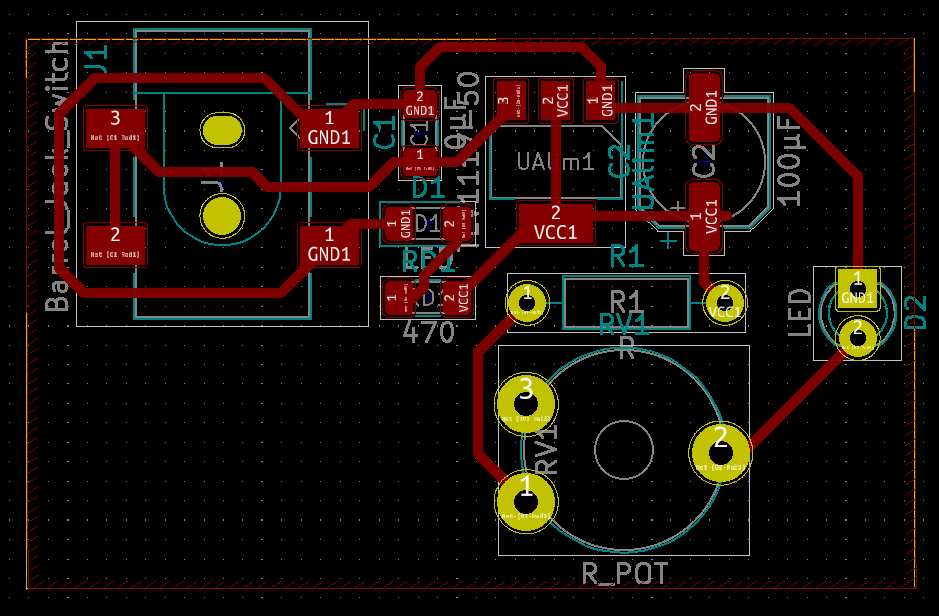
\includegraphics[scale=0.2]{figures/schema_pcb.png}
		\caption{\small{\textit{Schéma de la carte PCB}}}
		\label{fig:led_pcb}
	\end{subfigure}
	\caption{\small{\textit{Schéma Kicad et schéma de la PCB réalisés pour la LED}}}
	\label{fig:led}
\end{figure}
L’utilisation de la LED haute intensité permet de régler deux problèmes qui sont apparus lors de la mise en place. Premièrement, l’intensité obtenue sur l’écran est améliorée, ce qui permet une meilleure observation de l’effet Schlieren. Deuxièmement, l’utilisation de la LED et de la boîte permet une meilleure précision du montage et l’obtention d’une source ponctuelle qui accorde un meilleur filtrage avec la lame de rasoir. La lumière est également plus blanche qu’une lampe de téléphone, améliorant ainsi la netteté de l’image. L’intensité de cette dernière peut être réglée à l’aide d’un potentiomètre.
\section{Observations et conclusion}
\subsection{Observations et analyse}
Concernant le dispositif avec miroir sphérique, on peut observer différentes images liées à différents changements d’indice optique: d’une part le briquet libérant du butane sans combustion :\\
\begin{figure}[H]
	\centering
	\begin{subfigure}[t]{0.49\textwidth}
		\centering
		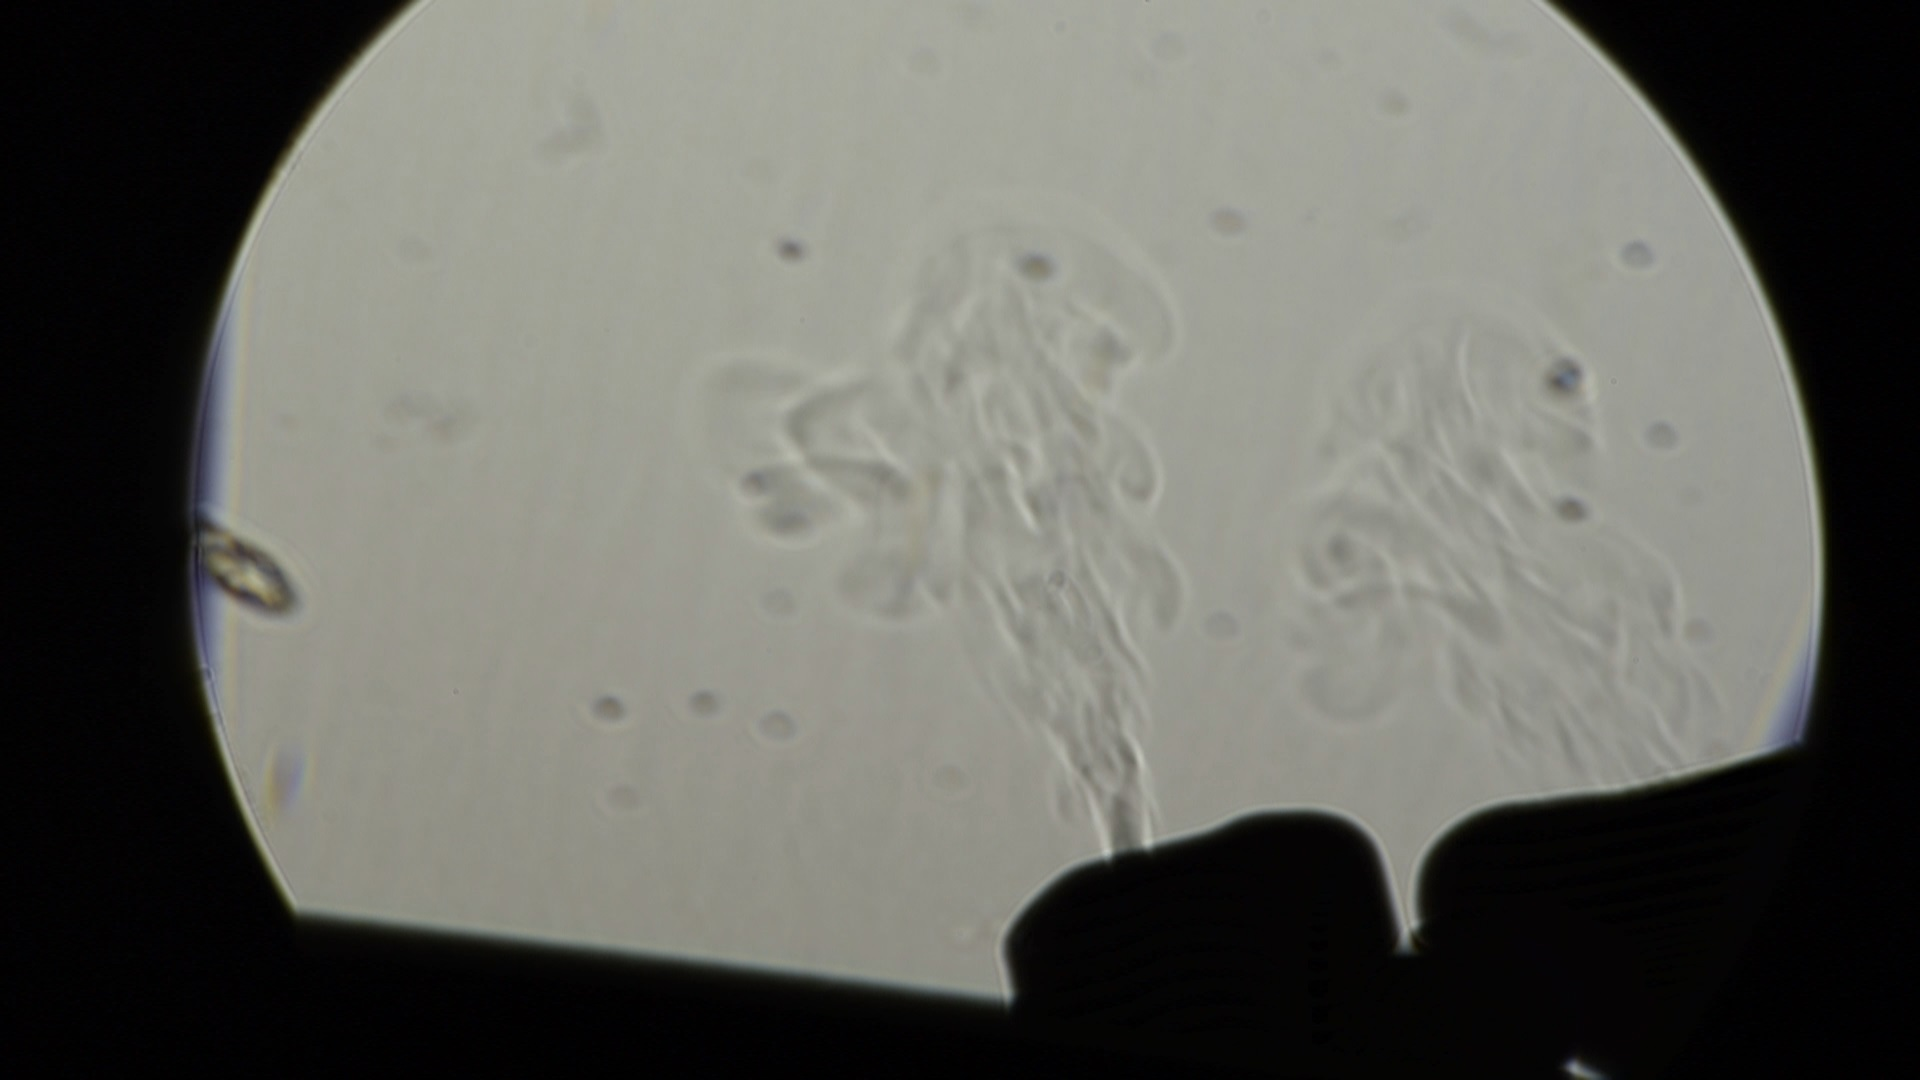
\includegraphics[scale=0.17]{figures/sans_combustion1.jpg}
		\label{fig:sans_combustion1}
	\end{subfigure}%
	\begin{subfigure}[t]{0.49\textwidth}
		\centering
		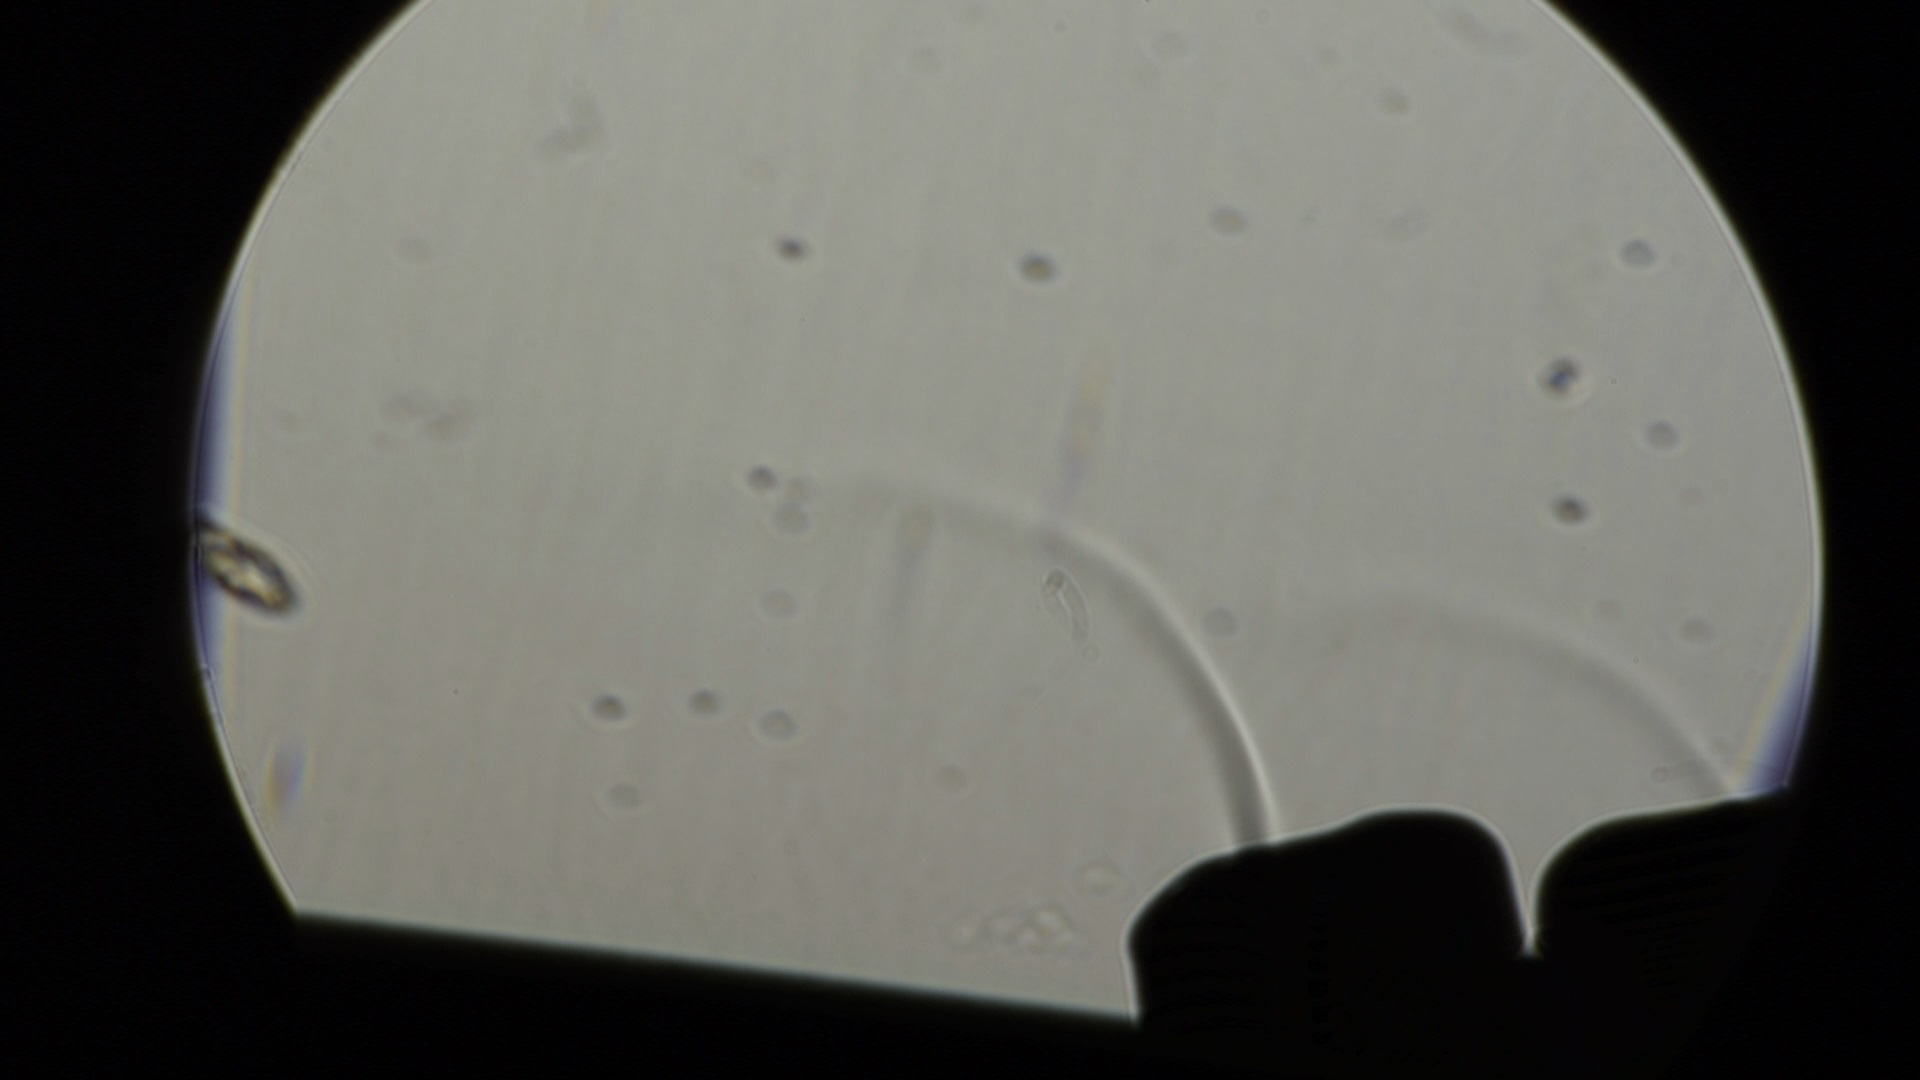
\includegraphics[scale=0.17]{figures/sans_combustion2.jpg}
		\label{fig:sans_combustion2}
	\end{subfigure}
	\caption{\small{\textit{Effet Schlieren observé sur un briquet sans combustion}}}
	\label{fig:briquet}
\end{figure}
d'autre part le même dispositif cette fois-ci avec combustion :\\
\begin{figure}[H]
	\centering
	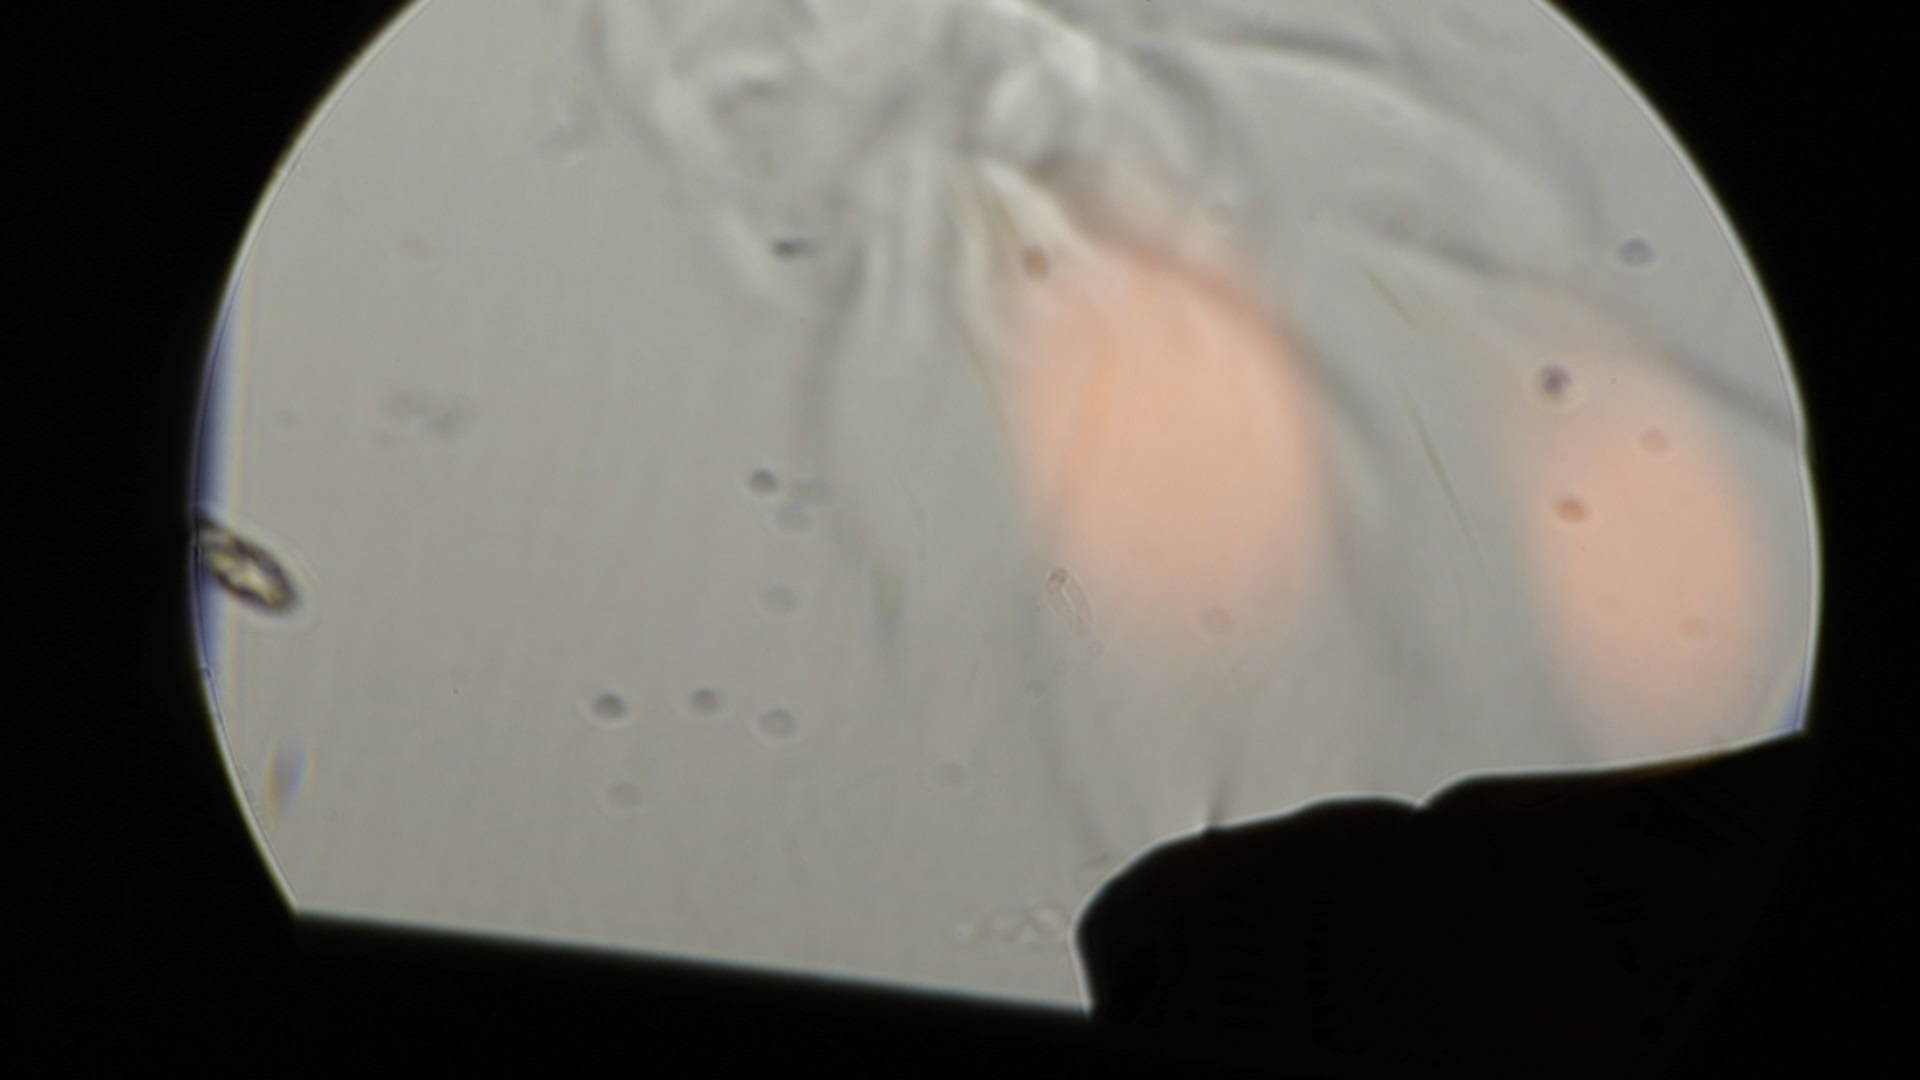
\includegraphics[scale = 0.17]{avec_combustion.jpg}
	\caption{\small{\textit{Effet Schlieren observé sur une flamme en combustion}}}
	\label{fig:avec_combustion}
\end{figure}
Sur la première image, on observe la propulsion du butane dans l’air engendrée par le briquet, puis sur la suivante le gaz se concentre de sorte à former un flux laminaire en apparence et dirigé vers le bas, ce qui s’explique par le fait que le butane est plus dense que l’air ($d$ = \textbf{2,29}). Lorsque la combustion apparaît, on observe le reflet de la lumière émise par la flamme sous forme de tâches oranges mais aussi le flux d’air chaud créé par la flamme. \\
La figure~\ref{fig:seche_cheveux} représente l'image obtenue par effet Schlieren sur un sèche-cheveux :
\begin{figure}[H]
	\centering
	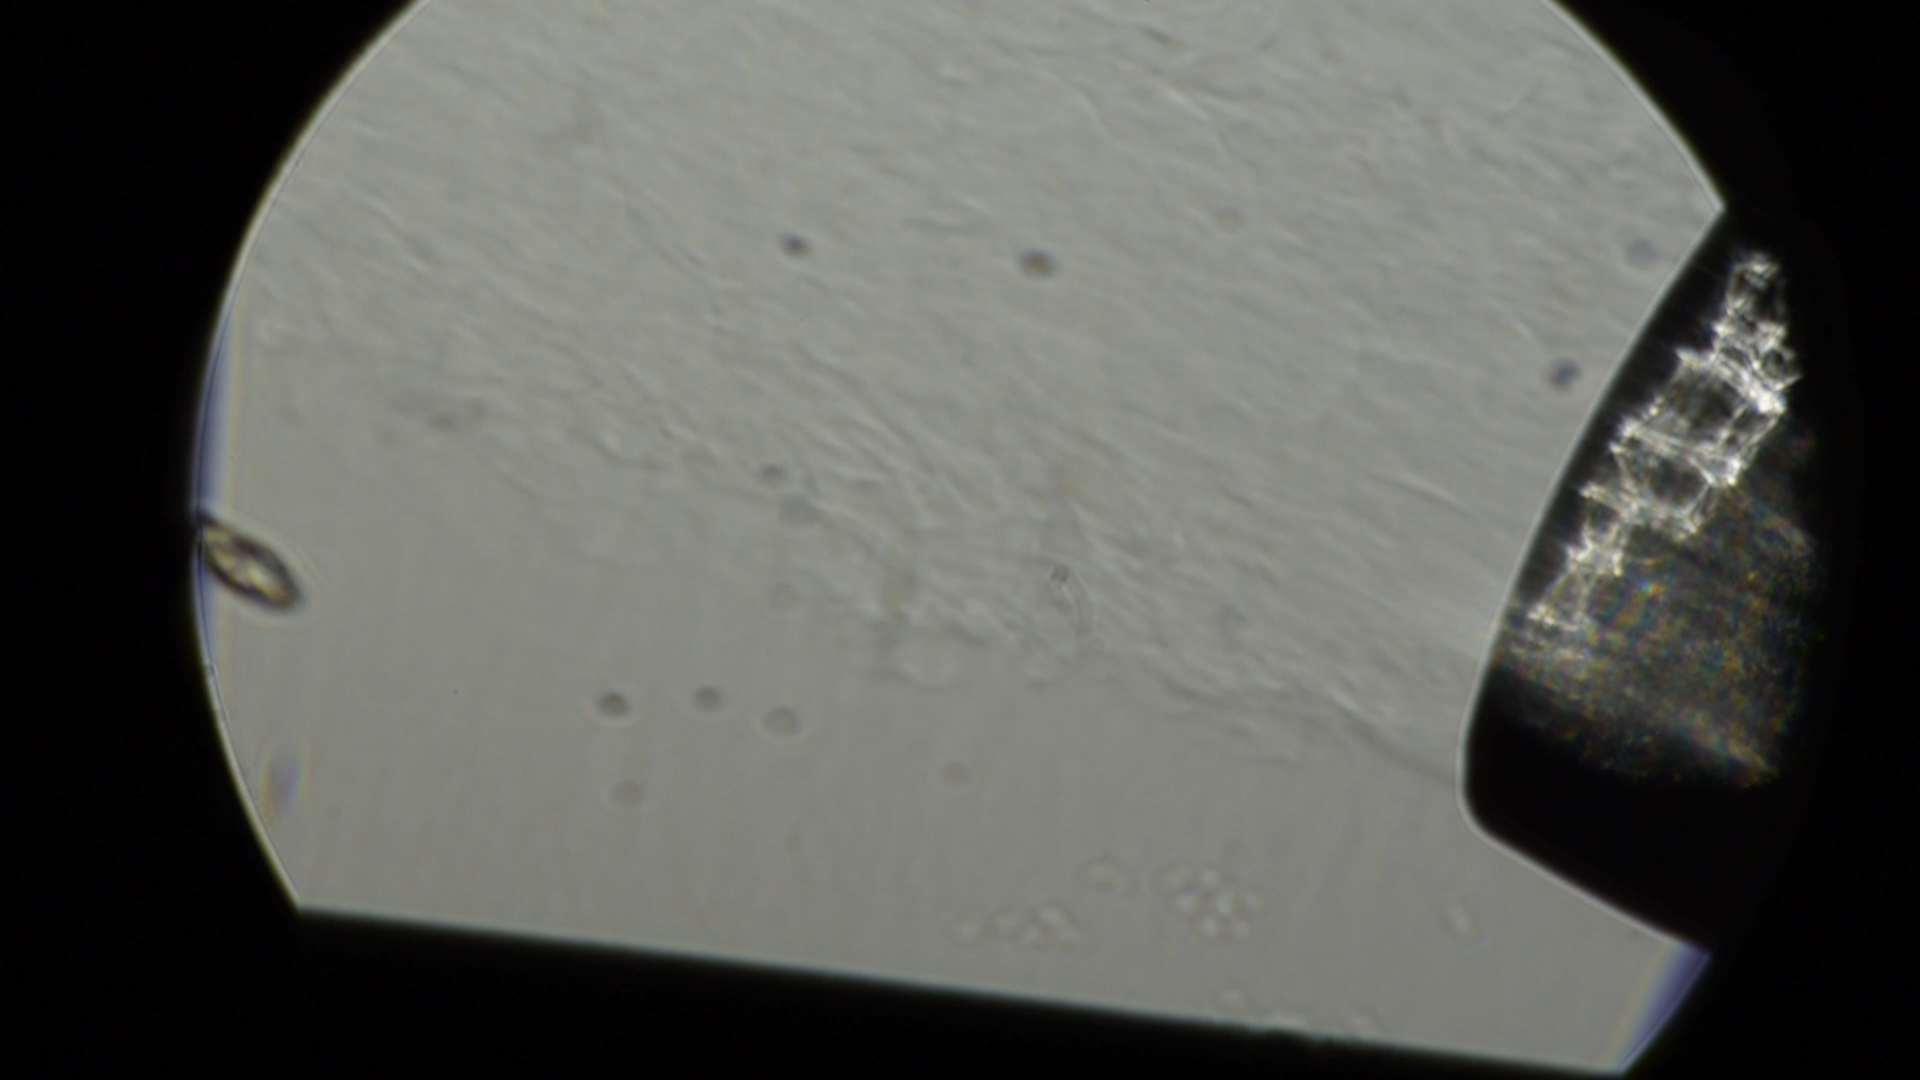
\includegraphics[scale = 0.17]{seche_cheveux.jpg}
	\caption{\small{\textit{Effet Schlieren observé sur l'air sortant d'un sèche-cheveux}}}
	\label{fig:seche_cheveux}
\end{figure}
Dans l’ensemble des calculs, on considère que les conditions initiales sont : \\
$T =$ \textbf{25 °C}, \,$P$ = \textbf{1 atm}, \,$\rho$ = \textbf{1,18} $Kg/m^{3}$, $k$ = \textbf{2,3}$\,\,\times\,10^{-4}\,\,m^{3}/Kg\,$ et on considère que l'air se comporte comme un gaz parfait.\\

Sachant que l’indice optique du butane est \textbf{$\mathnormal{n}$ = 1,443}~\ref{ref:techno_science}, la variation relative d’indice optique est de \textbf{44\,\%}, ce qui est en réalité observable sans dispositif particulier (l’eau a un indice optique de \textbf{1,33}). Néanmoins, le filtrage opéré permet de mieux mettre en évidence les détails.\\ \\
Le flux d’air chaud observé est quant à lui observable non pas grâce à un changement de molécules, mais grâce à un changement de masse volumique induit par un changement de température. Sachant que la température d'une flamme orange est autour de $T$=\textbf{1000 °C}, on peut en déduire la variation d'indice optique relative induite par cette variation de température :
\begin{align}
	\frac{\Delta n}{n}=\frac{n'-n}{n} \,&= \, k \,\,\frac{\rho' - \rho}{n}
	\label{indice_rho}\\
	|\rho' - \rho| \,&= \, P \,\,\frac{M}{R}\,\bigg{|}\frac{1}{T'}-\frac{1}{T}\bigg{|}
	\label{indice_pression}
\end{align}
En utilisant la relation des gaz parfaits :
\begin{align}
\frac{P}{\rho} = \frac{R\, T}{M}
\label{gaz_parfait}
\end{align}
on obtient, pour une flamme à $T$=\textbf{1000 °C}, une variation d'indice de :\\\\
\centerline{$\frac{\Delta n}{n} = $ \textbf{20,7\,\%}} \\\
Le sèche-cheveux induisant des variations de température plus faibles, il est plus difficile d’observer le flux de chaleur émis. En effet, en utilisant la relation des gaz parfait et en prenant une température \textbf{$T’$ = 90°C} pour le sèche-cheveux, on calcule la variation d'indice de réfraction à partir des relations~\ref{indice_rho} et~\ref{indice_pression}. On trouve finalement une variation relative d’indice optique de $\frac{\Delta n}{n}$ = \textbf{4,8\,\%}, bien plus faible que précédemment et non observable à l'œil nu.
\subsection{Comparaison des deux montages}
\subsubsection{\large\normalfont{\textsc{Montage avec lentilles convergentes}}}
Avec le dispositif des lentilles, le contraste n’est pas excellent. Cela est dû à la précision du montage qui est nettement moins bonne que celle du montage avec le miroir. En effet, l’utilisation de trois lentilles affecte la précision du montage et ainsi le rendu final. Le filtrage permet néanmoins une amélioration du contraste et améliore la qualité sur l’écran. Ce montage est correct pour des fortes variations d’indices notamment avec l’utilisation d’une flamme (briquet ou allumette). Cependant, avec le sèche-cheveux, les variations d’indices sont moins importantes car la température est plus faible que celle d’une flamme. De ce fait, on ne peut observer l’effet Schlieren avec ce montage. C’est pourquoi il est nécessaire d’utiliser un autre montage optique.
\subsubsection{\large\normalfont{\textsc{Montage avec miroir sphérique}}}
Avec le dispositif du miroir, le contraste est nettement meilleur, d'autant plus avec le filtrage. L’utilisation d’un seul élément optique permet une meilleure précision et ainsi un rendu très net. Cette fois-ci, nous pouvons observer nettement l’effet du sèche-cheveux sur la variation de l’indice de l’air. Il y a une réflexion totale de la lumière, ce qui permet d’obtenir une netteté plus importante. Pour améliorer ce rendu, nous pourrions utiliser des filtres de couleurs afin d’améliorer le contraste, mais cette solution ne sera pas détaillée ici.
\\
\\
Le tableau ci-dessous récapitule les différentes caractéristiques des deux montages :
\begin{table}[H]
	\centering
	\begin{tabular}{|l|l|l|}
		\hline
		&\small\textbf{{Montage avec miroir}}&\small\textbf{{Montage avec lentilles}}\\
		\hline
		\small{\textbf{Complexité du principe}}&\vtop{\hbox{\strut \small{Principe assez simple}}\hbox{\strut \small{à mettre en place}}}&\vtop{\hbox{\strut \small{Principe plus complexe}}\hbox{\strut \small{à mettre en place}}}\\
		\hline
		\small{\textbf{Contraste obtenu}}&\vtop{\hbox{\strut \small{Contraste bien visible,}}\hbox{\strut \small{images nettes}}}&\vtop{\hbox{\strut \small{Images moins nettes,}}\hbox{\strut \small{contraste pas très visible}}}\\
		\hline
		\small{\textbf{Objets observables}}&\vtop{\hbox{\strut \small{Flamme d'un briquet ou}}\hbox{\strut \small{d'une allumette, flux d'air }}\hbox{\strut \small{d'un sèche-cheveux}}}&\vtop{\hbox{\strut \small{Flamme d'un briquet ou}}\hbox{\strut \small{d'une allumette. Flux d'air}}\hbox{\strut \small{du sèche-cheveux non visible}}\hbox{\strut \small{à cause du faible contraste}}}\\
		\hline
		\small{\textbf{Coût du matériel}}&\small{Matériel coûteux}&\vtop{\hbox{\strut \small{Matériel moins coûteux}}\hbox{\strut \small{que le miroir sphérique}}}\\
		\hline
	\end{tabular}
	\caption{\small\textit{Tableau comparatif des deux montages optiques}}
	\label{fig:tableau_schlieren}
\end{table}
\subsection{Conclusion partielle}
En conclusion, la supériorité de qualité du montage avec miroir sphérique repose sur le fait que sa géométrie permet une bien meilleure convergence des rayons lumineux, cet avantage est d’autant plus marqué que la source est ponctuelle et que le filtrage bien opéré.
\\\\
Pour pousser encore plus loin l'intérêt de l’effet Schlieren, il a été décidé de réaliser un dispositif à onde de choc. Cette dernière provoque une variation de l’indice optique mais de manière très brève. Le dispositif en question couplé avec le montage optique Schlieren permet de visualiser nettement cette variation d’indice, et ainsi détecter la présence d’une onde de choc.  